\documentclass{article}
\usepackage[utf8]{inputenc}
\usepackage{amsmath,amssymb}
\usepackage[top=2cm, bottom=2cm, left=2cm, right=2cm]{geometry}
\usepackage[font=bf,figurename=Fig.,justification=centering]{caption}
\usepackage{graphicx,wrapfig,subcaption,adjustbox,tikz,float,biblatex}
\usepackage{url}

\bibliography{references.bib}


\pagenumbering{roman}

\title{Insurance Policy Pricing}
\author{Luke Dando}
\date{\today}

\begin{document}

\maketitle
\tableofcontents
\pagebreak
\pagenumbering{arabic}


\section{Distributions}
A probability distribution function, $p$, indicates the likelihood of an event or outcome. The following notation is generally used to describe said probabilities:
\begin{equation}
    p(x) = \text{the likelihood that random variable takes a specific value of x}.
\end{equation}

Intuitively, these distributions follow the exact principles one would assume to be true, in that:
\begin{enumerate}
    \item The sum of all probabilities muse be equal to $1$;
    \item Each particular value (or range of values) must be between $0$ and $1$.
\end{enumerate}

Generally, the properties of a distribution are laid out in a similar fashion:
\begin{itemize}
    \item \textbf{Variable}: usually, $X$ is used to denote random variables, and proceeds the important information about the distribution it is assigned to;
    \item \textbf{Tilde ($\mathbf{\sim}$)}: this is found immediately after the variable to indicate that it follows a distribution;
    \item \textbf{Distribution Identifier}: usually a capital letter, it identifies what distribution the following parameters are defining;
    \item \textbf{Parameters}: contained within parenthesis, these are important values that are used by the distribution model to behave in a desired manner.
\end{itemize}
This will become much clearer as you progress through the multiple distributions found in this section.

Each distribution can (usually) be partitioned into one of two groups: \textit{probability mass functions} or \textit{probability density functions}. It's not a tough task to figure out that they respectively hold values from either a discrete set or continuous set respectively. This detail is very important when it comes to deriving these functions, but for the most part we only need to know this so that we have an idea of what distribution can be used to model what set of data. 

\subsection{Continuous Distributions}
Continuous distributions are represented by probability mass functions (or PDFs for short)

\subsubsection{Uniform Distribution}
\begin{figure}[H]
\centering
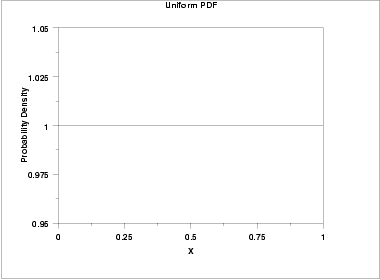
\includegraphics[width=0.5\textwidth]{images/unipdf.png}
\caption{Uniform Distribution}
\end{figure}

Perhaps the simplest of them all, uniform distribution is where the probability of any event that can occur is equally likely to any other. Mathematically speaking, we have
\begin{equation}
    f(x) = \frac{1}{B-A},\quad A\leq x \leq B.
\end{equation}
The case where $A=0$ and $B=1$ is called the \textbf{standard uniform distribution}.

\subsubsection{Normal Distribution}
\begin{figure}[H]
\centering
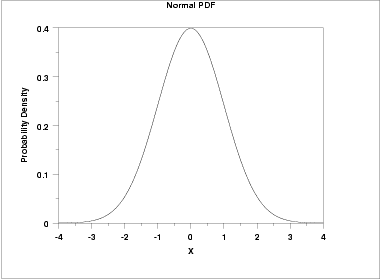
\includegraphics[width=0.5\textwidth]{images/norpdf.png}
\caption{Standard Normal Distribution} \label{fig:stand_norm_dis}
\end{figure}
A normal distribution, also referred to as a Gaussian distribution, is one of the most used commonly used distributions due to what is known as the central limit theorem, as well as its many uses within the sciences. It's function is defined as
\begin{equation}
    f(x) = \frac{1}{\sigma\sqrt{2\pi}}e^{-\frac{1}{2}\left( \frac{x-\mu}{\sigma} \right)^2}.
\end{equation}
Here, $\mu$ represents the mean, $\sigma$ is the standard deviation (with the variance being $\sigma^2$). This is usually written in the form of $X\sim N(\mu,\sigma^2)$.

A special case of this distribution is the \textbf{\textit{standard}} normal distribution seen in fig.~(\ref{fig:stand_norm_dis}). We set the variables to $\mu=0$ and $\sigma=1$, which simplifies the equation to
\begin{equation}
    f^*(x) = \frac{e^{-x^2/2}}{\sqrt{2\pi}}.
\end{equation}

\subsubsection{Gamma Distribution}
\begin{figure}[H]
\centering
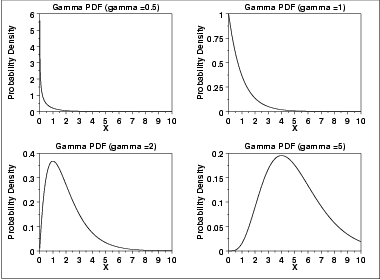
\includegraphics[width=0.5\textwidth]{images/gampdf4.png}
\caption{Several Standard Gamma Distributions} \label{fig:stand_gam_dis}
\end{figure}
The Gamma distribution is laid out similarly to the normal distribution as it is a two-parameter model which, when fixed, are important and well used special cases - just like the standard normal distribution. The function itself is defined as:
\begin{equation}
    f(x) = \frac{\left( \frac{x-\mu}{\beta} \right)^{\gamma -1}\exp{\left( -\frac{x-\mu}{\beta} \right)}}{\beta\Gamma(\gamma)},\quad x\geq\mu;\, \gamma,\beta>0,
\end{equation}
where $\gamma,\,\mu$ and $\beta$ are the shape, location and scale parameters respectively. Found in the denominator is the $\Gamma$ (Gamma) function; this is one of the most used `special' functions, finding it's way into many distributions and complex number equations. It is defined as:
\begin{equation}
    \Gamma(\alpha) = \int_0^\infty t^{\alpha-1}e^t\text{ d}t.
\end{equation}
As well as being the home of the exponential distribution, Erlang distribution, and chi-square distribution, it also has its own standard distribution just like the normal distribution; defined with $\mu=0$ and $\beta=1$. We can then vary the value of $\gamma$ to get distributions such as those found in fig.~(\ref{fig:stand_gam_dis})


\subsection{Discrete Distributions}
Discrete distributions are represented by probability mass functions (or PMFs for short)





\subsubsection{Normal Distribution}



\section{Risk}
\subsection{What is risk?}
Risk is the chance that something harmful or unexpected could occur regarding a held policy. This might involve loss, theft, or damage of valuable property and belongings, or it may involve someone being injured. From a statistical point-of-view risk can be defined as:
\begin{equation}
    \tau = \mathbb{E}\left[\frac{L}{e}\right].
\end{equation}
Here, $L$ is the loss and $e$ is the exposure of the policy. If we now assume that the frequency of a claim is independent from the severity of it (thus inferring $\mathbb{E}[XY] = \mathbb{E}[X]\mathbb{E}[Y]$), we find:
\begin{align}
    \tau &= \mathbb{E}\left[\frac{L}{e}\right], \\
    &= \mathbb{E}\left[ \left. \left( \frac{L}{N} \cdot\frac{N}{e} \right) \right\vert N>0 \right], \\
    &= \mathbb{E}\left[\left.\frac{L}{N}\right\vert N>0\right]\cdot\mathbb{E}\left[\frac{N}{e}\right], \\
    &= \mathbb{E}[F]\cdot\mathbb{E}[S],
\end{align}
where $N$ is the number of claims, $S$ is the severity (or size) of the claim and $F$ is the claim frequency.\\
This forms the basis of how our burn costs are set when defining our technical prices.

\section{Linear Models}
\subsection{Introducing the problem}
GLMs are generalized forms of linear models, so in order to understand them it would be ideal to first review classic linear models through an example. \\
Both these models have the same purpose: to determine the relationship between an observed response variable, $Y$, and predictor variables $X$. For example, let there be a total of $4$ predictor variables: we then define $Y$ as
\begin{equation}
    Y = \beta_1X_1 + \beta_2X_2 + \beta_3X_3 + \beta_4X_4 + \epsilon.
\end{equation}

\begin{table}[H]
\centering
\begin{tabular}{l|l|l|}
\cline{2-3}
                             & Urban & Rural \\ \hline
\multicolumn{1}{|l|}{Male}   & 800   & 500   \\ \hline
\multicolumn{1}{|l|}{Female} & 400   & 200   \\ \hline
\end{tabular}
    \caption{Covariances for linear model example.}
    \label{fig:covariances_example}
\end{table}

Here, $\epsilon$ is an error term, usually Normally distributed with mean zero and variance $\sigma^2$ (often written as $\epsilon~\sim~\mathcal{N}(0,\sigma^2)$). Our covariates will be representing male ($X_1$), female ($X_2$), urban ($X_3$) and rural ($X_4$). These and their respective values can be seen in table~\ref{fig:covariances_example}.\\
The problem here is that, with as many parameters as there are combinations of rating factor levels being considered and a linear dependency between the four, the model is not uniquely defined. In order to do so, we remove one of these parameters from our model, leaving us with
\begin{equation}
    Y = \beta_1X_1 + \beta_2X_2 + \beta_3X_3  + \epsilon. \label{eq:linear_model_1}
\end{equation}
We can express our observations as the following:
\begin{align}
    Y_1 &= 800 = \beta_1 + 0 + \beta_3 + \epsilon_1;\\
    Y_2 &= 500 = \beta_1 + 0 + 0 + \epsilon_2;\\
    Y_3 &= 400 = 0 + \beta_2 + \beta_3 + \epsilon_3;\\
    Y_4 &= 200 = \beta_2 + 0 + \epsilon_4.
\end{align}
We then want to find the best values for $\beta$, which we do so through minimizing the sum of squared errors (SSE):
\begin{align}
    SSE &= \epsilon_1^2 + \epsilon_2^2 + \epsilon_3^2 + \epsilon_4^2, \\
    &= (800-\beta_1-\beta_3)^2 + (500-\beta_1)^2 + (400-\beta_2 - \beta_3)^2 + (200-\beta_2)^2.
\end{align}
We can minimize this by setting the following system of equations
\begin{equation}
    \left.\frac{\partial SSE}{\partial \beta_i}\right\vert_{i=1,2,3} = 0.
\end{equation}
This is trivial enough and can be solved to derive:
\begin{align}
    \beta_1 = 525,\\ \label{eq:simp1}
    \beta_2 = 175,\\
    \beta_3 = 250.\label{eq:simp3}
\end{align}

\subsection{Vector and Matrix Notation}\label{sec:vec_not}
Let $\mathbf{Y}$ be a column vector with components corresponding to the observed values for the response variable:
\begin{equation}
    \underline{Y} = \begin{bmatrix} Y_1 \\ Y_2 \\ Y_3 \\ Y_4 \end{bmatrix} = \begin{bmatrix} 800 \\ 500 \\ 400 \\ 200 \end{bmatrix}
\end{equation}
Next, let $\underline{X}_1$, $\underline{X}_2$, $\underline{X}_3$ denote the column vectors with components equal to the observed values for the respective indicator variables (eg the $i$\textsuperscript{th} element of $\underline{X}_1$ is $1$ when the $i$\textsuperscript{th} observation is male, and $0$ if female):
\begin{equation}
    \underline{X}_1 = \begin{bmatrix} 1 \\ 1 \\ 0 \\ 0 \end{bmatrix},\qquad \underline{X}_2 = \begin{bmatrix} 0 \\ 0 \\ 1 \\ 1 \end{bmatrix},\qquad \underline{X}_3 = \begin{bmatrix} 1 \\ 0 \\ 1 \\ 0 \end{bmatrix}.
\end{equation}
We can then finally denote $\underline{\beta}$ and $\underline{\epsilon}$ as
\begin{equation}
    \underline{\beta}=\begin{bmatrix} \beta_1 \\ \beta_2 \\ \beta_3 \end{bmatrix},\qquad \underline{\epsilon}=\begin{bmatrix} \epsilon_1 \\ \epsilon_2 \\ \epsilon_3 \\ \epsilon_4 \end{bmatrix}.
\end{equation}
The system of equations can now take the form:
\begin{equation}
    \underline{Y} = \beta_1\underline{X}_1 + \beta_2\underline{X}_2 + \beta_3\underline{X}_3 + \underline{\epsilon}.
\end{equation}
We can further simplify this by aggregating $\underline{X}_1$, $\underline{X}_2$, $\underline{X}_3$ into a single matrix $\mathbf{X}$. This is called the \textbf{design matrix} and would (in this example) be defined as:
\begin{equation}
    \mathbf{X} = \begin{bmatrix} 1 & 0 & 1 \\ 1 & 0 & 0 \\ 0 & 1 & 1 \\ 0 & 1 & 0 \end{bmatrix}.
\end{equation}
We now find that the system of equations takes the form
\begin{equation}
    \underline{Y} = \mathbf{X}\cdot\underline{\beta} + \underline{\epsilon}.
\end{equation}

\subsection{Assumptions}
From the vectorized forms, we can determine the two elements required for a linear model
\begin{enumerate}
    \item a set of assumptions about the relationship between $\underline{Y}$ and the predictor variables,
    \item an objective function which is to be optimized in order to solve the problem. It can be shown outside of this material that the parameters which minimize the sum of squared error (SSE) also maximize the likelihood.
\end{enumerate}
Finally, we now make three explicit assumptions about the model:
\begin{itemize}
    \item \textbf{(LM1)} \textit{Random component}: Each component of \underline{Y} is independent and is Normally distributed. The mean, $\mu_i$, of each component is allowed to differ, but they all have common variance $\sigma^2$; 
    \item \textbf{(LM2)} \textit{Systematic component}: The $p$ covariates are combined to give the linear predictor $\underline{\eta}$:
\begin{equation}
    \underline{\eta} = \mathbf{X}\cdot\underline{\beta};
\end{equation}
\item \textbf{(LM3)} \textit{Link function}: The relationship between the random and systematic components is specified via a link function. In the linear model the link function is equal to the identity function so that:
\begin{equation}
    \mathbb{E}[\underline{Y}] \equiv \underline{\mu} = \underline{\eta}.
\end{equation}
\end{itemize}

\section{Generalized Linear Model}
A GLM allows for a non-linear dependence through what's called a link function, $g$:
\begin{equation}
    \mathbb{E}[\mathbf{Y}] = g^{-1}(\mathbf{X}\cdot\mathbf{\beta}).
\end{equation}
Here, $Y$ is the dependent variable, $X$ the independent variables and $\beta$ the parameters that are fitted through regression. 
\subsection{Assumptions}
There are three main assumptions that will form the foundation of our model building:
\begin{itemize}
    \item \textbf{Policy independence:} For $n$ considered policies, $X_1,\ldots,X_n$ are independent where $X_i$ denotes the response for policy $i$.\\
    There are some situations that obviously don't abide by this assumption (two Hastings Direct customers claiming against one another), but the effect of neglecting this should be small.
    \item \textbf{Time independence:} Consider $n$ disjoint time intervals. For any response type, let $X_i$ denote the response in time interval $i$. Then $X_1\ldots,X_n$ are independent.\\
    This essentially states that any amount of claims made in one time interval will not directly influence the number made in another. Although not entirely true, again it's a reasonable enough assumption to make in order to help simplify the calculations needed to create the statistical model.
    \item \textbf{Homogeneity:} Consider any two policies with the same exposure and the same 
\end{itemize}

\subsection{Simple examples}
We will solve simple examples using the same observations previously discussed in sec.~(\ref{sec:vec_not}). The general procedure for solving a GLM involves the following:
\begin{enumerate}
    \item Specify the matrix $\mathbf{X}$ and the vector of parameters $\underline{\beta}$;
    \item Choose the error structure and link function;
    \item Identify the log-likelihood function;
    \item Take the logarithm to convert the product of many terms into a sum;
    \item Maximize the logarithm of the likelihood function;
    \item Compute the predicted values.
\end{enumerate}
We will follow the following models:
\begin{itemize}
    \item Normal error structure with an identity link function.
    \item Poisson error structure with a log link function.
    \item Gamma error structure with an inverse link function.
\end{itemize}
Note that for these examples, the prior weights ($\underline{\omega}$) and the offset term ($\underline{\xi}$) are set to $1$ and $0$ respectively in order to simplify these calculations.




\subsubsection{Normal error structure with identity link function}
This is a good introductory example as it also shows where the link is between the $SSE$ and the likelihood function falls with regards to the classic linearization model. \\
The predicted values in this example will take the following form:
\begin{equation}
    \mathbb{E}[\underline{Y}] = g^{-1}(X\cdot \underline{\beta}) = \begin{bmatrix} g^{-1}(\beta_1 + \beta_3) \\ g^{-1}(\beta_1) \\ g^{-1}(\beta_2 + \beta_3) \\ g^{-1}(\beta_2) \end{bmatrix} = \begin{bmatrix} \beta_1 + \beta_3 \\ \beta_1 \\ \beta_2 + \beta_3 \\ \beta_2 \end{bmatrix}.
\end{equation}
Next, we can define our density function $f$ using our prior assumptions that the mean is $\mu$ and our variance is $\sigma^2$:
\begin{equation}
    f(y;\,\mu,\sigma^2) = \exp{\left\{ -\frac{(y_i-\mu_i)^2}{2\sigma^2}-\frac{1}{2}\ln{(2\pi\sigma^2)} \right\}}.
\end{equation}
Our likelihood function is then
\begin{equation}
    L(y;\,\mu,\sigma^2) = \prod_{i=1}^n\exp{\left\{ -\frac{(y_i-\mu_i)^2}{2\sigma^2}-\frac{1}{2}\ln{(2\pi\sigma^2)} \right\}}.
\end{equation}
We know that maximizing the likelihood function is equivalent to maximizing the log-likelihood function:
\begin{equation}
    \log(L(y;\,\mu,\sigma^2)) = l(y;\,\mu,\sigma^2) = \log\left(\prod_{i=1}^n\exp{\left\{ -\frac{(y_i-\mu_i)^2}{2\sigma^2}-\frac{1}{2}\ln{(2\pi\sigma^2)} \right\}}\right).\label{eq:log_like}
\end{equation}
We can use our fundamental laws of indices and products/summations to adapt 
\begin{equation}
    \prod_{i=1}^n e^{x_i} = e^{x_1}\cdot e^{x_2}\cdot\ldots\cdot e^{x_n} = e^{x_1+x_2+\ldots x_n} = e^{\sum_{i=1}^n x_i},
\end{equation}
and apply it to our log-likelihood found in eq.~(\ref{eq:log_like}). This gives us
\begin{equation}
    l(y;\,\mu,\sigma^2) = \sum_{i=1}^n -\frac{(y_i-\mu_i)^2}{2\sigma^2}-\frac{1}{2}\ln{(2\pi\sigma^2)}.
\end{equation}
Here, we insert our link function (identity link function in this case), $\mu_{ij}=\sum_jX_{ij}\beta_j$, to find
\begin{equation}
    l(y;\,\mu,\sigma^2) = \sum_{i=1}^n -\frac{\left(y_i-\sum_j X_{ij}\beta_j\right)^2}{2\sigma^2}-\frac{1}{2}\ln{(2\pi\sigma^2)}.
\end{equation}
We now expand the right hand side in order to observe
\begin{align}
    l(y;\,\mu,\sigma^2) &= -\frac{(800-(\beta_1+\beta_3))^2}{2\sigma^2} -\frac{(500-\beta_1)^2}{2\sigma^2}-\frac{(400-(\beta_2+\beta_3))^2}{2\sigma^2}-\frac{(200-\beta_2)^2}{2\sigma^2} - 2\ln(2\pi\sigma^2), \\
    l^*(y;\,\mu,\sigma^2) &= -\frac{(800-(\beta_1+\beta_3))^2}{2\sigma^2} -\frac{(500-\beta_1)^2}{2\sigma^2}-\frac{(400-(\beta_2+\beta_3))^2}{2\sigma^2}-\frac{(200-\beta_2)^2}{2\sigma^2},
\end{align}
which is up to that constant we ``removed'' ($2\ln(2\sigma^2)$).\\
To maximize $l^*$, we take derivatives with respect to $\beta_1$, $\beta_2$ and $\beta_3$ and then setting them to zero.
\begin{align}
    \frac{\partial l^*}{\partial \beta_1} &= 0 \implies \beta_1 + \beta_3 + \beta_1 = 800+500+1300; \\
    \frac{\partial l^*}{\partial \beta_2} &= 0 \implies \beta_2 + \beta_3 + \beta_2 = 400 + 200 = 600\\
    \frac{\partial l^*}{\partial \beta_3} &= 0 \implies \beta_1 + \beta_3 + \beta_2 + \beta_3 = 800+400 = 1200.
\end{align}
You can now see how these equations are identical to those that would be found in the simple linear model. These again are solved to derive:
\begin{align}
    \beta_1 = 525; \\
    \beta_2 = 175; \\
    \beta_3 = 250.
\end{align}
These are the same as the solutions found in eq.~(\ref{eq:simp1}-\ref{eq:simp3}). This in turn produces the following predicted values:
\begin{table}[H]
\centering
\begin{tabular}{l|l|l|}
\cline{2-3}
                             & Urban & Rural \\ \hline
\multicolumn{1}{|l|}{Male}   & 775   & 525   \\ \hline
\multicolumn{1}{|l|}{Female} & 425   & 175   \\ \hline
\end{tabular}
    \caption{Predicted values using the Normal error structure with identity link function.}
    \label{fig:covariances_example_1}
\end{table}

\subsubsection{The Poisson error structure with a logarithmic link function}
For our Poisson model, we begin with our predicted values:
\begin{equation}
    \mathbb{E}[\underline{Y}] = g^{-1}(X\cdot \underline{\beta}) = \begin{bmatrix} g^{-1}(\beta_1 + \beta_3) \\ g^{-1}(\beta_1) \\ g^{-1}(\beta_2 + \beta_3) \\ g^{-1}(\beta_2) \end{bmatrix} = \begin{bmatrix} e^{\beta_1 + \beta_3} \\ e^{\beta_1} \\ e^{\beta_2 + \beta_3} \\ e^{\beta_2} \end{bmatrix}.
\end{equation}
Using the Poisson distribution density function  ($f(y;\,\mu)=e^{-\mu}\mu^y/y!$), we can introduce the log-likelihood function as
\begin{equation}
    l(y;\,\mu) = \sum_{i=1}^n \ln f(y;\,\mu) = \sum_{i=1}^n-\mu_i + y_i\ln\mu_i-\ln(y_i!).
\end{equation}
We then introduce the link function which in this case is the logarithmic link function $\mu_i = \exp{(\sum_j X_{ij}\beta_j)}$. This reduces the log-likelihood function to
\begin{equation}
    l(y;\,e^{X\beta}) = \sum_{i=1}^n-\exp{(\sum_j X_{ij}\beta_j)} + y_i\sum_j X_{ij}\beta_j-\ln(y_i!).
\end{equation}
We can (however tedious) expand this into
\begin{align}
    l(y;\,\mu) = &-e^{(\beta_1+\beta_3)}+800\cdot(\beta_1+\beta_3)-\ln{800!}-e^{\beta_1} + 500\cdot\beta_1 - \ln{500!} \nonumber \\ &\quad- e^{(\beta_2+\beta_3)}+400\cdot (\beta_2+\beta_3)-\ln{400!} - e^{\beta_2}+200\cdot{\beta_2}-\ln{200!}.
\end{align}
Ignoring the constant, the following function is to be maximized:
\begin{equation}
    l^*(y;\,\mu) = -e^{(\beta_1+\beta_3)}+800\cdot(\beta_1+\beta_3)-e^{\beta_1} + 500\cdot\beta_1- e^{(\beta_2+\beta_3)}+400\cdot (\beta_2+\beta_3) - e^{\beta_2}+200\cdot{\beta_2}.
\end{equation}
To maximize $l^*$, the derivatives with respect to $\beta_{1,2,3}$ are set to zero and the following three equations are derived:
\begin{align}
    \frac{\partial l^*}{\partial\beta_1} &= 0 \implies e^{\beta_1}\cdot(e^{\beta_3}+1) = 1300,\\
    \frac{\partial l^*}{\partial\beta_2} &= 0 \implies e^{\beta_2}\cdot(e^{\beta_3}+1) = 600,\\
    \frac{\partial l^*}{\partial\beta_3} &= 0 \implies e^{\beta_3}\cdot(e^{\beta_1}+e^{\beta_2}) = 1200.
\end{align}
We can solve this system of equations to derive the following parameter estimates:
\begin{align}
    \beta_1 = 6.1716, \\
    \beta_2 = 5.3984, \\
    \beta_3 = 0.5390,
\end{align}
which in turn produces the following predicted values:
\begin{table}[H]
\centering
\begin{tabular}{l|l|l|}
\cline{2-3}
                             & Urban & Rural \\ \hline
\multicolumn{1}{|l|}{Male}   & 821.1   & 479.0   \\ \hline
\multicolumn{1}{|l|}{Female} & 378.9   & 221.1   \\ \hline
\end{tabular}
    \caption{Predicted values using the Poisson error structure with logarithmic link function.}
    \label{fig:covariances_example_2}
\end{table}

\subsubsection{The Gamma error structure with an inverse link function}
A Gamma distribution is substantially more difficult that the prior two examples, so feel free to skip it if it is out of the scope of your prior knowledge. \\
For the Gamma error structure, the predicted values take the form:
\begin{equation}
    \mathbb{E}[\underline{Y}] = g^{-1}(X\cdot \underline{\beta}) = \begin{bmatrix} g^{-1}(\beta_1 + \beta_3) \\ g^{-1}(\beta_1) \\ g^{-1}(\beta_2 + \beta_3) \\ g^{-1}(\beta_2) \end{bmatrix} = \begin{bmatrix} (\beta_1 + \beta_3)^{-1} \\ (\beta_1)^{-1} \\ (\beta_2 + \beta_3)^{-1} \\ (\beta_2)^{-1} \end{bmatrix}.
\end{equation}
The gamma error structure has the following density function:
\begin{equation}
    f(x;\,\mu,\phi) = \frac{x^{-1}}{\Gamma(1/\phi)}\left( \frac{x}{\mu\phi} \right)^{1/\phi}e^{\left( -\frac{x}{\mu\phi} \right)}.
\end{equation}
It's log-likelihood function is derived as 
\begin{equation}
    l(x;\,\mu,\phi) = \sum_{i=1}^n\frac{1}{\phi}\left( \ln{\frac{x_i}{\mu_i}} - \frac{x_i}{\mu_i} \right)-\ln{x_i} - \frac{\ln{\phi}}{\phi} - \ln{\Gamma\left( \frac{1}{\phi} \right)}.
\end{equation}
We can then introduce our inverse link function, $\mu_i = 1/(\sum_j X_{ij}\beta_j)$, to reduce the log-likelihood function to
\begin{equation}
    l(x;\,1/X\beta,\phi) = \sum_{i=1}^n \frac{1}{\phi}\left( \ln{\left( x_i\cdot\sum_{j=1}^p X_{ij}\beta_j \right)}-x_i\cdot\sum_{j=1}^p X_{ij}\beta_j \right)-\ln{x_i} -\frac{\ln{\phi}}{\phi} - \ln{\Gamma\left( \frac{1}{\phi} \right)}.
\end{equation}
This is then expanded to
\begin{align}
    l(x;\,\mu) = &\frac{1}{\phi}(\ln{(800\cdot(\beta_1+\beta_3))} - 800\cdot(\beta_1+\beta_3)) - \ln{800} - \frac{\ln{\phi}}{\phi} - \ln{\Gamma \left( \frac{1}{\phi} \right)} \nonumber \\
    &\quad+ \frac{1}{\phi}(\ln{(500\cdot(\beta_1))} - 500\cdot(\beta_1)) - \ln{500} - \frac{\ln{\phi}}{\phi} - \ln{\Gamma \left( \frac{1}{\phi} \right)} \nonumber \\
    &\quad+ \frac{1}{\phi}(\ln{(400\cdot(\beta_2+\beta_3))} - 400\cdot(\beta_2+\beta_3)) - \ln{400} - \frac{\ln{\phi}}{\phi} - \ln{\Gamma \left( \frac{1}{\phi} \right)} \nonumber \\
    &\quad+ \frac{1}{\phi}(\ln{(200\cdot(\beta_2))} - 200\cdot(\beta_2)) - \ln{200} - \frac{\ln{\phi}}{\phi} - \ln{\Gamma \left( \frac{1}{\phi} \right)}.
\end{align}
If we again ignore the constant terms (after multiplying by $\phi$), we then maximize the following function:
\begin{align}
    l^*(x;\,\mu) = &\ln{(800\cdot(\beta_1+\beta_3))} - 800\cdot(\beta_1+\beta_3) + 
    \ln{(500\cdot\beta_1)} - 500\cdot\beta_1) \nonumber\\
    &\quad+ \ln{(400\cdot(\beta_2+\beta_3))} - 400\cdot(\beta_2+\beta_3) + \ln{(200\cdot\beta_2)} - 200\cdot\beta_2.
\end{align}
To maximize $l^*$, the derivatives with respect to $\beta_{1,2,3}$ are set to zero and the following three equations are derived:
\begin{align}
    \frac{\partial l^*}{\partial\beta_1} &= 0 \implies \frac{1}{\beta_1+\beta_3}+\beta_1 = 1300,\\
    \frac{\partial l^*}{\partial\beta_2} &= 0 \implies \frac{1}{\beta_2+\beta_3}+\frac{1}{\beta_2}=600,\\
    \frac{\partial l^*}{\partial\beta_3} &= 0 \implies \frac{1}{\beta_1+\beta_3}+\frac{1}{\beta_2+\beta_3}=1200.
\end{align}
Solving these gives the following:
\begin{align}
    \beta_1 &= 0.00223804,\\
    \beta_2 &= 0.00394964,\\
    \beta_3 &= -0.00106601,
\end{align}
which results in the following predicted values:
\begin{table}[H]
\centering
\begin{tabular}{l|l|l|}
\cline{2-3}
                             & Urban & Rural \\ \hline
\multicolumn{1}{|l|}{Male}   & 853.2   & 446.8   \\ \hline
\multicolumn{1}{|l|}{Female} & 346.8   & 253.2   \\ \hline
\end{tabular}
    \caption{Predicted values using the Gamma error structure with inverse link function.}
    \label{fig:covariances_example_3}
\end{table}

\subsection{The Tweedie Distribution}
Modelling premiums can often be problematic, with one main problem being the high frequency of no-claims causing a large spike at zero and a wide range of amounts following on from this. May other more commonly taught distributions don't accurately account for this. In order to understand how this distribution is derived, we must break down what these distributions are attempting to model.

We essentially want to model the number of claims received, $N$, against the size of these claims, $Z_i$. Respectively, these can be accurately modelled through a Poisson distribution with mean $\lambda_i w_i$ ($N\sim P(\lambda_i w_i)$) and a gamma distribution with mean $\tau_i = \alpha\beta_i$ and shape parameter $\alpha$ ($\beta$ represents a rate parameter of our distribution). Therefore, we define our random variable $Z$ as the following:
\begin{equation}
    Z = \left\{ \begin{matrix} 0, & \text{if }N = 0, \\ \sum_{i=1}^N Z_i, & \text{if }N>0. \end{matrix}\right.
\end{equation}
This will evidently take into account the fact that if $N=0$ (No policy claims made), then the claim amount will \textit{also} be zero.

\subsection{Large Datasets and Numerical Techniques}
As the number of observations being modelled increases, the practicality of finding values of $\underline{\beta}$ which maximize likelihood using an explicit technique becomes less and less. Although there is a general case for solving the GLM problem using an assumed exponential distribution, we will now turn to numerical techniques to aid us in approaching our optimum.

\nocite{2008APG}
\nocite{géron2019hands}
\nocite{GLM_basics}
\printbibliography

\end{document}
